\documentclass[1p]{elsarticle_modified}
%\bibliographystyle{elsarticle-num}

%\usepackage[colorlinks]{hyperref}
%\usepackage{abbrmath_seonhwa} %\Abb, \Ascr, \Acal ,\Abf, \Afrak
\usepackage{amsfonts}
\usepackage{amssymb}
\usepackage{amsmath}
\usepackage{amsthm}
\usepackage{scalefnt}
\usepackage{amsbsy}
\usepackage{kotex}
\usepackage{caption}
\usepackage{subfig}
\usepackage{color}
\usepackage{graphicx}
\usepackage{xcolor} %% white, black, red, green, blue, cyan, magenta, yellow
\usepackage{float}
\usepackage{setspace}
\usepackage{hyperref}

\usepackage{tikz}
\usetikzlibrary{arrows}

\usepackage{multirow}
\usepackage{array} % fixed length table
\usepackage{hhline}

%%%%%%%%%%%%%%%%%%%%%
\makeatletter
\renewcommand*\env@matrix[1][\arraystretch]{%
	\edef\arraystretch{#1}%
	\hskip -\arraycolsep
	\let\@ifnextchar\new@ifnextchar
	\array{*\c@MaxMatrixCols c}}
\makeatother %https://tex.stackexchange.com/questions/14071/how-can-i-increase-the-line-spacing-in-a-matrix
%%%%%%%%%%%%%%%

\usepackage[normalem]{ulem}

\newcommand{\msout}[1]{\ifmmode\text{\sout{\ensuremath{#1}}}\else\sout{#1}\fi}
%SOURCE: \msout is \stkout macro in https://tex.stackexchange.com/questions/20609/strikeout-in-math-mode

\newcommand{\cancel}[1]{
	\ifmmode
	{\color{red}\msout{#1}}
	\else
	{\color{red}\sout{#1}}
	\fi
}

\newcommand{\add}[1]{
	{\color{blue}\uwave{#1}}
}

\newcommand{\replace}[2]{
	\ifmmode
	{\color{red}\msout{#1}}{\color{blue}\uwave{#2}}
	\else
	{\color{red}\sout{#1}}{\color{blue}\uwave{#2}}
	\fi
}

\newcommand{\Sol}{\mathcal{S}} %segment
\newcommand{\D}{D} %diagram
\newcommand{\A}{\mathcal{A}} %arc


%%%%%%%%%%%%%%%%%%%%%%%%%%%%%5 test

\def\sl{\operatorname{\textup{SL}}(2,\Cbb)}
\def\psl{\operatorname{\textup{PSL}}(2,\Cbb)}
\def\quan{\mkern 1mu \triangleright \mkern 1mu}

\theoremstyle{definition}
\newtheorem{thm}{Theorem}[section]
\newtheorem{prop}[thm]{Proposition}
\newtheorem{lem}[thm]{Lemma}
\newtheorem{ques}[thm]{Question}
\newtheorem{cor}[thm]{Corollary}
\newtheorem{defn}[thm]{Definition}
\newtheorem{exam}[thm]{Example}
\newtheorem{rmk}[thm]{Remark}
\newtheorem{alg}[thm]{Algorithm}

\newcommand{\I}{\sqrt{-1}}
\begin{document}

%\begin{frontmatter}
%
%\title{Boundary parabolic representations of knots up to 8 crossings}
%
%%% Group authors per affiliation:
%\author{Yunhi Cho} 
%\address{Department of Mathematics, University of Seoul, Seoul, Korea}
%\ead{yhcho@uos.ac.kr}
%
%
%\author{Seonhwa Kim} %\fnref{s_kim}}
%\address{Center for Geometry and Physics, Institute for Basic Science, Pohang, 37673, Korea}
%\ead{ryeona17@ibs.re.kr}
%
%\author{Hyuk Kim}
%\address{Department of Mathematical Sciences, Seoul National University, Seoul 08826, Korea}
%\ead{hyukkim@snu.ac.kr}
%
%\author{Seokbeom Yoon}
%\address{Department of Mathematical Sciences, Seoul National University, Seoul, 08826,  Korea}
%\ead{sbyoon15@snu.ac.kr}
%
%\begin{abstract}
%We find all boundary parabolic representation of knots up to 8 crossings.
%
%\end{abstract}
%\begin{keyword}
%    \MSC[2010] 57M25 
%\end{keyword}
%
%\end{frontmatter}

%\linenumbers
%\tableofcontents
%
\newcommand\colored[1]{\textcolor{white}{\rule[-0.35ex]{0.8em}{1.4ex}}\kern-0.8em\color{red} #1}%
%\newcommand\colored[1]{\textcolor{white}{ #1}\kern-2.17ex	\textcolor{white}{ #1}\kern-1.81ex	\textcolor{white}{ #1}\kern-2.15ex\color{red}#1	}

{\Large $\underline{12a_{0833}~(K12a_{0833})}$}

\setlength{\tabcolsep}{10pt}
\renewcommand{\arraystretch}{1.6}
\vspace{1cm}\begin{tabular}{m{100pt}>{\centering\arraybackslash}m{274pt}}
\multirow{5}{120pt}{
	\centering
	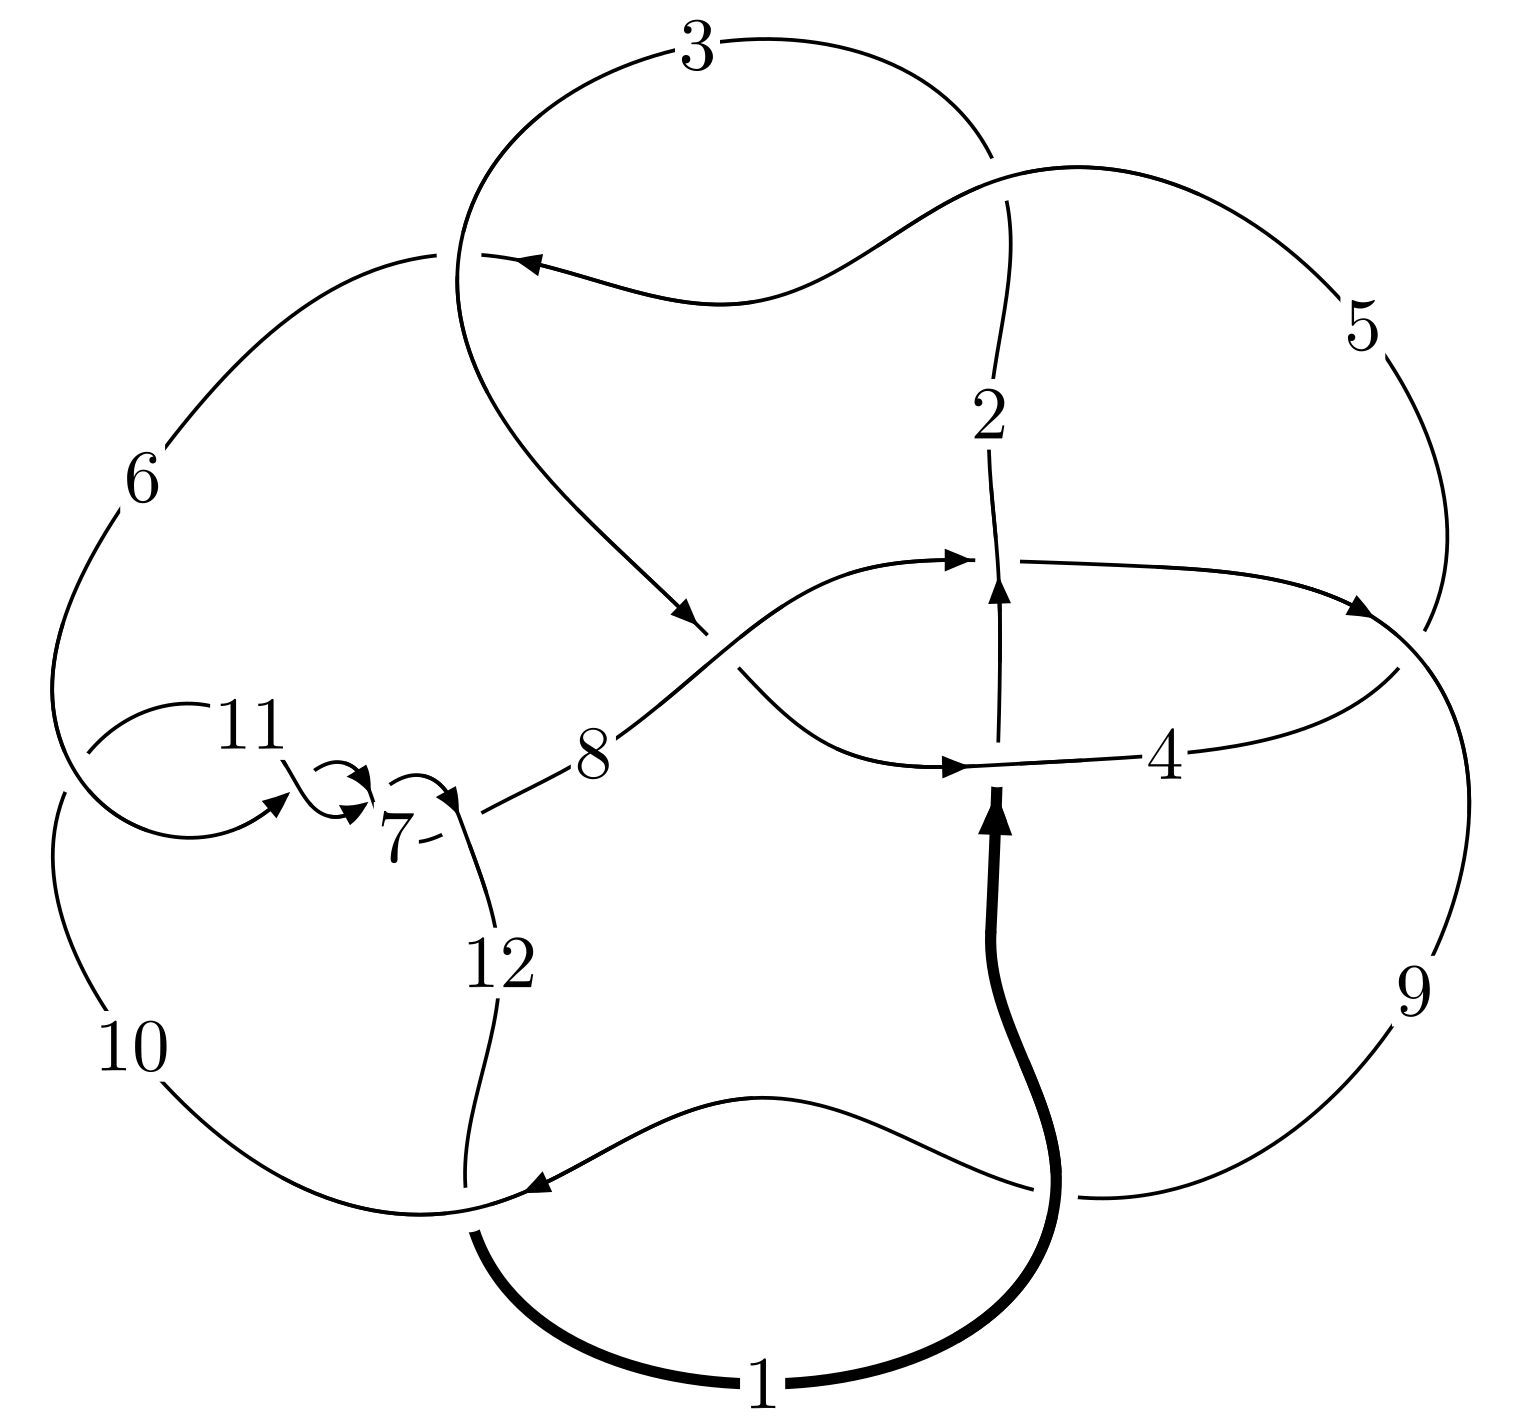
\includegraphics[width=112pt]{../../../GIT/diagram.site/Diagrams/png/1634_12a_0833.png}\\
\ \ \ A knot diagram\footnotemark}&
\allowdisplaybreaks
\textbf{Linearized knot diagam} \\
\cline{2-2}
 &
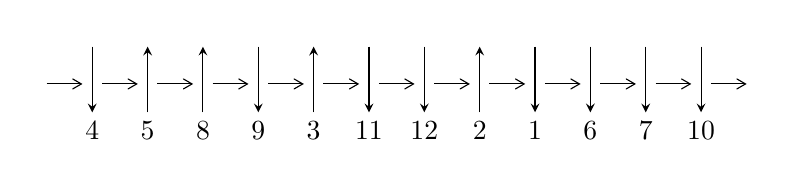
\begin{tikzpicture}[x=20pt, y=17pt]
	% nodes
	\node (C0) at (0, 0) {};
	\node (C1) at (1, 0) {};
	\node (C1U) at (1, +1) {};
	\node (C1D) at (1, -1) {4};

	\node (C2) at (2, 0) {};
	\node (C2U) at (2, +1) {};
	\node (C2D) at (2, -1) {5};

	\node (C3) at (3, 0) {};
	\node (C3U) at (3, +1) {};
	\node (C3D) at (3, -1) {8};

	\node (C4) at (4, 0) {};
	\node (C4U) at (4, +1) {};
	\node (C4D) at (4, -1) {9};

	\node (C5) at (5, 0) {};
	\node (C5U) at (5, +1) {};
	\node (C5D) at (5, -1) {3};

	\node (C6) at (6, 0) {};
	\node (C6U) at (6, +1) {};
	\node (C6D) at (6, -1) {11};

	\node (C7) at (7, 0) {};
	\node (C7U) at (7, +1) {};
	\node (C7D) at (7, -1) {12};

	\node (C8) at (8, 0) {};
	\node (C8U) at (8, +1) {};
	\node (C8D) at (8, -1) {2};

	\node (C9) at (9, 0) {};
	\node (C9U) at (9, +1) {};
	\node (C9D) at (9, -1) {1};

	\node (C10) at (10, 0) {};
	\node (C10U) at (10, +1) {};
	\node (C10D) at (10, -1) {6};

	\node (C11) at (11, 0) {};
	\node (C11U) at (11, +1) {};
	\node (C11D) at (11, -1) {7};

	\node (C12) at (12, 0) {};
	\node (C12U) at (12, +1) {};
	\node (C12D) at (12, -1) {10};
	\node (C13) at (13, 0) {};

	% arrows
	\draw[->,>={angle 60}]
	(C0) edge (C1) (C1) edge (C2) (C2) edge (C3) (C3) edge (C4) (C4) edge (C5) (C5) edge (C6) (C6) edge (C7) (C7) edge (C8) (C8) edge (C9) (C9) edge (C10) (C10) edge (C11) (C11) edge (C12) (C12) edge (C13) ;	\draw[->,>=stealth]
	(C1U) edge (C1D) (C2D) edge (C2U) (C3D) edge (C3U) (C4U) edge (C4D) (C5D) edge (C5U) (C6U) edge (C6D) (C7U) edge (C7D) (C8D) edge (C8U) (C9U) edge (C9D) (C10U) edge (C10D) (C11U) edge (C11D) (C12U) edge (C12D) ;
	\end{tikzpicture} \\
\hhline{~~} \\& 
\textbf{Solving Sequence} \\ \cline{2-2} 
 &
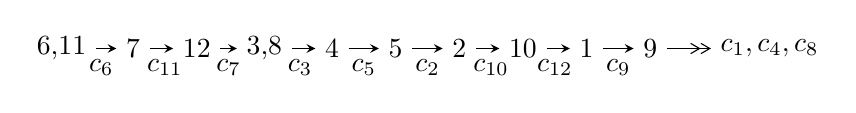
\begin{tikzpicture}[x=23pt, y=7pt]
	% node
	\node (A0) at (-1/8, 0) {6,11};
	\node (A1) at (1, 0) {7};
	\node (A2) at (2, 0) {12};
	\node (A3) at (49/16, 0) {3,8};
	\node (A4) at (33/8, 0) {4};
	\node (A5) at (41/8, 0) {5};
	\node (A6) at (49/8, 0) {2};
	\node (A7) at (57/8, 0) {10};
	\node (A8) at (65/8, 0) {1};
	\node (A9) at (73/8, 0) {9};
	\node (C1) at (1/2, -1) {$c_{6}$};
	\node (C2) at (3/2, -1) {$c_{11}$};
	\node (C3) at (5/2, -1) {$c_{7}$};
	\node (C4) at (29/8, -1) {$c_{3}$};
	\node (C5) at (37/8, -1) {$c_{5}$};
	\node (C6) at (45/8, -1) {$c_{2}$};
	\node (C7) at (53/8, -1) {$c_{10}$};
	\node (C8) at (61/8, -1) {$c_{12}$};
	\node (C9) at (69/8, -1) {$c_{9}$};
	\node (A10) at (11, 0) {$c_{1},c_{4},c_{8}$};

	% edge
	\draw[->,>=stealth]	
	(A0) edge (A1) (A1) edge (A2) (A2) edge (A3) (A3) edge (A4) (A4) edge (A5) (A5) edge (A6) (A6) edge (A7) (A7) edge (A8) (A8) edge (A9) ;
	\draw[->>,>={angle 60}]	
	(A9) edge (A10);
\end{tikzpicture} \\ 

\end{tabular} \\

\footnotetext{
The image of knot diagram is generated by the software ``\textbf{Draw programme}" developed by Andrew Bartholomew(\url{http://www.layer8.co.uk/maths/draw/index.htm\#Running-draw}), where we modified some parts for our purpose(\url{https://github.com/CATsTAILs/LinksPainter}).
}\phantom \\ \newline 
\centering \textbf{Ideals for irreducible components\footnotemark of $X_{\text{par}}$} 
 
\begin{align*}
I^u_{1}&=\langle 
6.92226\times10^{23} u^{76}+2.25852\times10^{24} u^{75}+\cdots+3.76421\times10^{24} b+1.44507\times10^{24},\\
\phantom{I^u_{1}}&\phantom{= \langle  }-8.36115\times10^{24} u^{76}-3.47813\times10^{25} u^{75}+\cdots+3.76421\times10^{24} a+4.23354\times10^{25},\;u^{77}+2 u^{76}+\cdots+u+1\rangle \\
I^u_{2}&=\langle 
b-1,\;a- u-3,\;u^2+u-1\rangle \\
\\
\end{align*}
\raggedright * 2 irreducible components of $\dim_{\mathbb{C}}=0$, with total 79 representations.\\
\footnotetext{All coefficients of polynomials are rational numbers. But the coefficients are sometimes approximated in decimal forms when there is not enough margin.}
\newpage
\renewcommand{\arraystretch}{1}
\centering \section*{I. $I^u_{1}= \langle 6.92\times10^{23} u^{76}+2.26\times10^{24} u^{75}+\cdots+3.76\times10^{24} b+1.45\times10^{24},\;-8.36\times10^{24} u^{76}-3.48\times10^{25} u^{75}+\cdots+3.76\times10^{24} a+4.23\times10^{25},\;u^{77}+2 u^{76}+\cdots+u+1 \rangle$}
\flushleft \textbf{(i) Arc colorings}\\
\begin{tabular}{m{7pt} m{180pt} m{7pt} m{180pt} }
\flushright $a_{6}=$&$\begin{pmatrix}1\\0\end{pmatrix}$ \\
\flushright $a_{11}=$&$\begin{pmatrix}0\\u\end{pmatrix}$ \\
\flushright $a_{7}=$&$\begin{pmatrix}1\\u^2\end{pmatrix}$ \\
\flushright $a_{12}=$&$\begin{pmatrix}- u\\- u^3+u\end{pmatrix}$ \\
\flushright $a_{3}=$&$\begin{pmatrix}2.22122 u^{76}+9.24000 u^{75}+\cdots-29.9150 u-11.2468\\-0.183897 u^{76}-0.599998 u^{75}+\cdots+1.78805 u-0.383897\end{pmatrix}$ \\
\flushright $a_{8}=$&$\begin{pmatrix}- u^2+1\\- u^4+2 u^2\end{pmatrix}$ \\
\flushright $a_{4}=$&$\begin{pmatrix}2.46730 u^{76}+6.84009 u^{75}+\cdots-19.3082 u-7.80666\\0.0679123 u^{76}-1.39991 u^{75}+\cdots+6.03396 u+1.46791\end{pmatrix}$ \\
\flushright $a_{5}=$&$\begin{pmatrix}-1.93121 u^{76}-8.43999 u^{75}+\cdots+27.5519 u+11.3966\\0.264412 u^{76}+0.600009 u^{75}+\cdots-1.84779 u+0.464412\end{pmatrix}$ \\
\flushright $a_{2}=$&$\begin{pmatrix}1.23607 u^{76}+1.79998 u^{75}+\cdots-5.48564 u-0.683416\\0.838969 u^{76}-0.0000226859 u^{75}+\cdots+0.119485 u+0.838970\end{pmatrix}$ \\
\flushright $a_{10}=$&$\begin{pmatrix}u\\u\end{pmatrix}$ \\
\flushright $a_{1}=$&$\begin{pmatrix}u^5-2 u^3- u\\u^5-3 u^3+u\end{pmatrix}$ \\
\flushright $a_{9}=$&$\begin{pmatrix}u^9-4 u^7+3 u^5+2 u^3+u\\u^9-5 u^7+7 u^5-2 u^3+u\end{pmatrix}$\\&\end{tabular}
\flushleft \textbf{(ii) Obstruction class $= -1$}\\~\\
\flushleft \textbf{(iii) Cusp Shapes $= \frac{18898874875970222080511766}{3764208987280068409379969} u^{76}+\frac{23036948754797654651395635}{3764208987280068409379969} u^{75}+\cdots+\frac{89792714215852879307532136}{3764208987280068409379969} u+\frac{28083545111696464689731405}{3764208987280068409379969}$}\\~\\
\newpage\renewcommand{\arraystretch}{1}
\flushleft \textbf{(iv) u-Polynomials at the component}\newline \\
\begin{tabular}{m{50pt}|m{274pt}}
Crossings & \hspace{64pt}u-Polynomials at each crossing \\
\hline $$\begin{aligned}c_{1}\end{aligned}$$&$\begin{aligned}
&u^{77}-13 u^{76}+\cdots+28 u-4
\end{aligned}$\\
\hline $$\begin{aligned}c_{2},c_{5}\end{aligned}$$&$\begin{aligned}
&u^{77}+3 u^{76}+\cdots-28 u-1
\end{aligned}$\\
\hline $$\begin{aligned}c_{3}\end{aligned}$$&$\begin{aligned}
&u^{77}+2 u^{76}+\cdots+36927 u-10649
\end{aligned}$\\
\hline $$\begin{aligned}c_{4}\end{aligned}$$&$\begin{aligned}
&u^{77}+46 u^{75}+\cdots-3159 u-521
\end{aligned}$\\
\hline $$\begin{aligned}c_{6},c_{7},c_{10}\\c_{11}\end{aligned}$$&$\begin{aligned}
&u^{77}-2 u^{76}+\cdots+u-1
\end{aligned}$\\
\hline $$\begin{aligned}c_{8}\end{aligned}$$&$\begin{aligned}
&u^{77}-4 u^{76}+\cdots- u+1
\end{aligned}$\\
\hline $$\begin{aligned}c_{9},c_{12}\end{aligned}$$&$\begin{aligned}
&u^{77}-12 u^{76}+\cdots-7323 u+937
\end{aligned}$\\
\hline
\end{tabular}\\~\\
\newpage\renewcommand{\arraystretch}{1}
\flushleft \textbf{(v) Riley Polynomials at the component}\newline \\
\begin{tabular}{m{50pt}|m{274pt}}
Crossings & \hspace{64pt}Riley Polynomials at each crossing \\
\hline $$\begin{aligned}c_{1}\end{aligned}$$&$\begin{aligned}
&y^{77}+15 y^{76}+\cdots+8 y-16
\end{aligned}$\\
\hline $$\begin{aligned}c_{2},c_{5}\end{aligned}$$&$\begin{aligned}
&y^{77}-59 y^{76}+\cdots+840 y-1
\end{aligned}$\\
\hline $$\begin{aligned}c_{3}\end{aligned}$$&$\begin{aligned}
&y^{77}+36 y^{76}+\cdots+7037007165 y-113401201
\end{aligned}$\\
\hline $$\begin{aligned}c_{4}\end{aligned}$$&$\begin{aligned}
&y^{77}+92 y^{76}+\cdots+6188485 y-271441
\end{aligned}$\\
\hline $$\begin{aligned}c_{6},c_{7},c_{10}\\c_{11}\end{aligned}$$&$\begin{aligned}
&y^{77}-84 y^{76}+\cdots+9 y-1
\end{aligned}$\\
\hline $$\begin{aligned}c_{8}\end{aligned}$$&$\begin{aligned}
&y^{77}-16 y^{76}+\cdots+9 y-1
\end{aligned}$\\
\hline $$\begin{aligned}c_{9},c_{12}\end{aligned}$$&$\begin{aligned}
&y^{77}+60 y^{76}+\cdots-6663999 y-877969
\end{aligned}$\\
\hline
\end{tabular}\\~\\
\newpage\flushleft \textbf{(vi) Complex Volumes and Cusp Shapes}
$$\begin{array}{c|c|c}  
\text{Solutions to }I^u_{1}& \I (\text{vol} + \sqrt{-1}CS) & \text{Cusp shape}\\
 \hline 
\begin{aligned}
u &= \phantom{-}0.853925 + 0.296160 I \\
a &= \phantom{-}0.973281 - 0.595252 I \\
b &= \phantom{-}1.172540 + 0.189613 I\end{aligned}
 & \phantom{-}1.07224 + 1.58898 I & \phantom{-0.000000 } 0 \\ \hline\begin{aligned}
u &= \phantom{-}0.853925 - 0.296160 I \\
a &= \phantom{-}0.973281 + 0.595252 I \\
b &= \phantom{-}1.172540 - 0.189613 I\end{aligned}
 & \phantom{-}1.07224 - 1.58898 I & \phantom{-0.000000 } 0 \\ \hline\begin{aligned}
u &= -0.593838 + 0.645320 I \\
a &= -0.63075 + 1.51672 I \\
b &= \phantom{-}1.270780 + 0.133216 I\end{aligned}
 & \phantom{-}7.55124 + 4.72924 I & \phantom{-0.000000 } 0. - 6.30385 I \\ \hline\begin{aligned}
u &= -0.593838 - 0.645320 I \\
a &= -0.63075 - 1.51672 I \\
b &= \phantom{-}1.270780 - 0.133216 I\end{aligned}
 & \phantom{-}7.55124 - 4.72924 I & \phantom{-0.000000 -}0. + 6.30385 I \\ \hline\begin{aligned}
u &= \phantom{-}0.581242 + 0.631919 I \\
a &= -1.12909 - 2.01443 I \\
b &= \phantom{-}1.44071 - 0.50854 I\end{aligned}
 & \phantom{-}8.3310 - 13.1724 I & \phantom{-0.000000 -}0. + 9.15625 I \\ \hline\begin{aligned}
u &= \phantom{-}0.581242 - 0.631919 I \\
a &= -1.12909 + 2.01443 I \\
b &= \phantom{-}1.44071 + 0.50854 I\end{aligned}
 & \phantom{-}8.3310 + 13.1724 I & \phantom{-0.000000 } 0. - 9.15625 I \\ \hline\begin{aligned}
u &= -0.766915 + 0.349815 I \\
a &= \phantom{-}0.45233 + 1.81840 I \\
b &= \phantom{-}1.257950 + 0.389125 I\end{aligned}
 & \phantom{-}1.58579 + 7.91925 I & -4.00000 - 9.21393 I \\ \hline\begin{aligned}
u &= -0.766915 - 0.349815 I \\
a &= \phantom{-}0.45233 - 1.81840 I \\
b &= \phantom{-}1.257950 - 0.389125 I\end{aligned}
 & \phantom{-}1.58579 - 7.91925 I & -4.00000 + 9.21393 I \\ \hline\begin{aligned}
u &= \phantom{-}0.546540 + 0.601133 I \\
a &= \phantom{-}1.244280 + 0.506121 I \\
b &= -0.172494 + 1.220390 I\end{aligned}
 & \phantom{-}3.24579 - 7.19707 I & -1.99256 + 9.26795 I \\ \hline\begin{aligned}
u &= \phantom{-}0.546540 - 0.601133 I \\
a &= \phantom{-}1.244280 - 0.506121 I \\
b &= -0.172494 - 1.220390 I\end{aligned}
 & \phantom{-}3.24579 + 7.19707 I & -1.99256 - 9.26795 I\\
 \hline 
 \end{array}$$\newpage$$\begin{array}{c|c|c}  
\text{Solutions to }I^u_{1}& \I (\text{vol} + \sqrt{-1}CS) & \text{Cusp shape}\\
 \hline 
\begin{aligned}
u &= \phantom{-}0.511919 + 0.613048 I \\
a &= \phantom{-}1.43493 + 1.72189 I \\
b &= -1.55248 + 0.63641 I\end{aligned}
 & \phantom{-}7.52474 - 4.19900 I & \phantom{-}4.30781 + 6.64099 I \\ \hline\begin{aligned}
u &= \phantom{-}0.511919 - 0.613048 I \\
a &= \phantom{-}1.43493 - 1.72189 I \\
b &= -1.55248 - 0.63641 I\end{aligned}
 & \phantom{-}7.52474 + 4.19900 I & \phantom{-}4.30781 - 6.64099 I \\ \hline\begin{aligned}
u &= -0.401184 + 0.687267 I \\
a &= -0.832182 + 0.272529 I \\
b &= \phantom{-}1.287680 - 0.080245 I\end{aligned}
 & \phantom{-}8.12227 - 0.25245 I & \phantom{-}4.74578 - 0.31294 I \\ \hline\begin{aligned}
u &= -0.401184 - 0.687267 I \\
a &= -0.832182 - 0.272529 I \\
b &= \phantom{-}1.287680 + 0.080245 I\end{aligned}
 & \phantom{-}8.12227 + 0.25245 I & \phantom{-}4.74578 + 0.31294 I \\ \hline\begin{aligned}
u &= \phantom{-}0.411672 + 0.667315 I \\
a &= -0.830610 - 0.220703 I \\
b &= \phantom{-}1.44202 + 0.47832 I\end{aligned}
 & \phantom{-}8.83402 + 8.79252 I & \phantom{-}0.88977 - 3.35804 I \\ \hline\begin{aligned}
u &= \phantom{-}0.411672 - 0.667315 I \\
a &= -0.830610 + 0.220703 I \\
b &= \phantom{-}1.44202 - 0.47832 I\end{aligned}
 & \phantom{-}8.83402 - 8.79252 I & \phantom{-}0.88977 + 3.35804 I \\ \hline\begin{aligned}
u &= -0.529363 + 0.577415 I \\
a &= -0.135208 - 0.789858 I \\
b &= -0.209697 - 0.347656 I\end{aligned}
 & \phantom{-}3.14595 + 2.98011 I & -2.41069 - 2.46896 I \\ \hline\begin{aligned}
u &= -0.529363 - 0.577415 I \\
a &= -0.135208 + 0.789858 I \\
b &= -0.209697 + 0.347656 I\end{aligned}
 & \phantom{-}3.14595 - 2.98011 I & -2.41069 + 2.46896 I \\ \hline\begin{aligned}
u &= \phantom{-}0.480416 + 0.616913 I \\
a &= \phantom{-}0.579023 + 0.909776 I \\
b &= -1.58087 - 0.58209 I\end{aligned}
 & \phantom{-}7.61770 + 0.01954 I & \phantom{-}4.76574 + 0.17184 I \\ \hline\begin{aligned}
u &= \phantom{-}0.480416 - 0.616913 I \\
a &= \phantom{-}0.579023 - 0.909776 I \\
b &= -1.58087 + 0.58209 I\end{aligned}
 & \phantom{-}7.61770 - 0.01954 I & \phantom{-}4.76574 - 0.17184 I\\
 \hline 
 \end{array}$$\newpage$$\begin{array}{c|c|c}  
\text{Solutions to }I^u_{1}& \I (\text{vol} + \sqrt{-1}CS) & \text{Cusp shape}\\
 \hline 
\begin{aligned}
u &= -0.494713 + 0.592724 I \\
a &= \phantom{-}3.16136 - 1.21835 I \\
b &= -1.125500 - 0.016130 I\end{aligned}
 & \phantom{-}5.08899 + 2.02411 I & -19.3118 - 1.4800 I \\ \hline\begin{aligned}
u &= -0.494713 - 0.592724 I \\
a &= \phantom{-}3.16136 + 1.21835 I \\
b &= -1.125500 + 0.016130 I\end{aligned}
 & \phantom{-}5.08899 - 2.02411 I & -19.3118 + 1.4800 I \\ \hline\begin{aligned}
u &= \phantom{-}0.438086 + 0.613550 I \\
a &= -0.671045 + 0.081730 I \\
b &= -0.234394 - 1.182410 I\end{aligned}
 & \phantom{-}3.56479 + 3.06303 I & -0.82722 - 2.95608 I \\ \hline\begin{aligned}
u &= \phantom{-}0.438086 - 0.613550 I \\
a &= -0.671045 - 0.081730 I \\
b &= -0.234394 + 1.182410 I\end{aligned}
 & \phantom{-}3.56479 - 3.06303 I & -0.82722 + 2.95608 I \\ \hline\begin{aligned}
u &= -0.454585 + 0.581796 I \\
a &= -0.700983 + 0.414818 I \\
b &= -0.299545 + 0.306129 I\end{aligned}
 & \phantom{-}3.36686 + 0.99145 I & -1.25975 - 4.73968 I \\ \hline\begin{aligned}
u &= -0.454585 - 0.581796 I \\
a &= -0.700983 - 0.414818 I \\
b &= -0.299545 - 0.306129 I\end{aligned}
 & \phantom{-}3.36686 - 0.99145 I & -1.25975 + 4.73968 I \\ \hline\begin{aligned}
u &= -0.662313 + 0.211934 I \\
a &= \phantom{-}0.35497 - 1.59761 I \\
b &= \phantom{-}0.052783 - 0.855449 I\end{aligned}
 & -2.18565 + 3.46642 I & -10.30084 - 8.03918 I \\ \hline\begin{aligned}
u &= -0.662313 - 0.211934 I \\
a &= \phantom{-}0.35497 + 1.59761 I \\
b &= \phantom{-}0.052783 + 0.855449 I\end{aligned}
 & -2.18565 - 3.46642 I & -10.30084 + 8.03918 I \\ \hline\begin{aligned}
u &= \phantom{-}0.582849 + 0.322676 I \\
a &= -1.21537 - 0.97656 I \\
b &= \phantom{-}0.305951 - 0.408414 I\end{aligned}
 & -1.56034 - 0.79420 I & -10.59198 + 4.32165 I \\ \hline\begin{aligned}
u &= \phantom{-}0.582849 - 0.322676 I \\
a &= -1.21537 + 0.97656 I \\
b &= \phantom{-}0.305951 + 0.408414 I\end{aligned}
 & -1.56034 + 0.79420 I & -10.59198 - 4.32165 I\\
 \hline 
 \end{array}$$\newpage$$\begin{array}{c|c|c}  
\text{Solutions to }I^u_{1}& \I (\text{vol} + \sqrt{-1}CS) & \text{Cusp shape}\\
 \hline 
\begin{aligned}
u &= -0.036520 + 0.599242 I \\
a &= -0.827030 + 0.013934 I \\
b &= \phantom{-}1.257970 - 0.282910 I\end{aligned}
 & \phantom{-}3.88684 - 4.68919 I & \phantom{-}2.22512 + 5.21190 I \\ \hline\begin{aligned}
u &= -0.036520 - 0.599242 I \\
a &= -0.827030 - 0.013934 I \\
b &= \phantom{-}1.257970 + 0.282910 I\end{aligned}
 & \phantom{-}3.88684 + 4.68919 I & \phantom{-}2.22512 - 5.21190 I \\ \hline\begin{aligned}
u &= \phantom{-}0.563481\phantom{ +0.000000I} \\
a &= -0.745038\phantom{ +0.000000I} \\
b &= \phantom{-}0.0349557\phantom{ +0.000000I}\end{aligned}
 & -0.922835\phantom{ +0.000000I} & -10.6560\phantom{ +0.000000I} \\ \hline\begin{aligned}
u &= \phantom{-}1.42367 + 0.20238 I \\
a &= \phantom{-}0.304978 - 0.285826 I \\
b &= \phantom{-}1.311050 + 0.004533 I\end{aligned}
 & \phantom{-}2.29463 - 2.93841 I & \phantom{-0.000000 } 0 \\ \hline\begin{aligned}
u &= \phantom{-}1.42367 - 0.20238 I \\
a &= \phantom{-}0.304978 + 0.285826 I \\
b &= \phantom{-}1.311050 - 0.004533 I\end{aligned}
 & \phantom{-}2.29463 + 2.93841 I & \phantom{-0.000000 } 0 \\ \hline\begin{aligned}
u &= -1.44300 + 0.19292 I \\
a &= \phantom{-}0.428691 - 0.138349 I \\
b &= \phantom{-}1.44221 - 0.43358 I\end{aligned}
 & \phantom{-}2.88358 - 5.72307 I & \phantom{-0.000000 } 0 \\ \hline\begin{aligned}
u &= -1.44300 - 0.19292 I \\
a &= \phantom{-}0.428691 + 0.138349 I \\
b &= \phantom{-}1.44221 + 0.43358 I\end{aligned}
 & \phantom{-}2.88358 + 5.72307 I & \phantom{-0.000000 } 0 \\ \hline\begin{aligned}
u &= -0.481253 + 0.252904 I \\
a &= -0.87479 - 2.48795 I \\
b &= -1.085940 - 0.463047 I\end{aligned}
 & \phantom{-}1.84563 + 2.21443 I & -1.06316 - 9.09042 I \\ \hline\begin{aligned}
u &= -0.481253 - 0.252904 I \\
a &= -0.87479 + 2.48795 I \\
b &= -1.085940 + 0.463047 I\end{aligned}
 & \phantom{-}1.84563 - 2.21443 I & -1.06316 + 9.09042 I \\ \hline\begin{aligned}
u &= -1.48480 + 0.16334 I \\
a &= -0.928276 + 0.982359 I \\
b &= -0.330290 + 1.148720 I\end{aligned}
 & -2.68476 - 0.33795 I & \phantom{-0.000000 } 0\\
 \hline 
 \end{array}$$\newpage$$\begin{array}{c|c|c}  
\text{Solutions to }I^u_{1}& \I (\text{vol} + \sqrt{-1}CS) & \text{Cusp shape}\\
 \hline 
\begin{aligned}
u &= -1.48480 - 0.16334 I \\
a &= -0.928276 - 0.982359 I \\
b &= -0.330290 - 1.148720 I\end{aligned}
 & -2.68476 + 0.33795 I & \phantom{-0.000000 } 0 \\ \hline\begin{aligned}
u &= \phantom{-}1.49604\phantom{ +0.000000I} \\
a &= -1.27137\phantom{ +0.000000I} \\
b &= -1.51544\phantom{ +0.000000I}\end{aligned}
 & -3.24017\phantom{ +0.000000I} & \phantom{-0.000000 } 0 \\ \hline\begin{aligned}
u &= \phantom{-}0.492260 + 0.077362 I \\
a &= -2.26092 + 6.41672 I \\
b &= -0.953862 + 0.013143 I\end{aligned}
 & \phantom{-}0.798661 - 0.174787 I & \phantom{-}27.8903 - 10.4954 I \\ \hline\begin{aligned}
u &= \phantom{-}0.492260 - 0.077362 I \\
a &= -2.26092 - 6.41672 I \\
b &= -0.953862 - 0.013143 I\end{aligned}
 & \phantom{-}0.798661 + 0.174787 I & \phantom{-}27.8903 + 10.4954 I \\ \hline\begin{aligned}
u &= \phantom{-}1.50405 + 0.15591 I \\
a &= -1.037770 - 0.828109 I \\
b &= -0.415857 - 0.300870 I\end{aligned}
 & -3.06301 - 3.56838 I & \phantom{-0.000000 } 0 \\ \hline\begin{aligned}
u &= \phantom{-}1.50405 - 0.15591 I \\
a &= -1.037770 + 0.828109 I \\
b &= -0.415857 + 0.300870 I\end{aligned}
 & -3.06301 + 3.56838 I & \phantom{-0.000000 } 0 \\ \hline\begin{aligned}
u &= -1.50575 + 0.17891 I \\
a &= -0.822676 - 0.369551 I \\
b &= -1.61992 + 0.52632 I\end{aligned}
 & \phantom{-}1.10913 + 2.81557 I & \phantom{-0.000000 } 0 \\ \hline\begin{aligned}
u &= -1.50575 - 0.17891 I \\
a &= -0.822676 + 0.369551 I \\
b &= -1.61992 - 0.52632 I\end{aligned}
 & \phantom{-}1.10913 - 2.81557 I & \phantom{-0.000000 } 0 \\ \hline\begin{aligned}
u &= \phantom{-}1.51956 + 0.04330 I \\
a &= -1.33810 + 1.94670 I \\
b &= -1.010310 + 0.705360 I\end{aligned}
 & -4.84400 - 3.13283 I & \phantom{-0.000000 } 0 \\ \hline\begin{aligned}
u &= \phantom{-}1.51956 - 0.04330 I \\
a &= -1.33810 - 1.94670 I \\
b &= -1.010310 - 0.705360 I\end{aligned}
 & -4.84400 + 3.13283 I & \phantom{-0.000000 } 0\\
 \hline 
 \end{array}$$\newpage$$\begin{array}{c|c|c}  
\text{Solutions to }I^u_{1}& \I (\text{vol} + \sqrt{-1}CS) & \text{Cusp shape}\\
 \hline 
\begin{aligned}
u &= \phantom{-}1.51829 + 0.17105 I \\
a &= \phantom{-}1.87369 + 1.53109 I \\
b &= -1.129620 + 0.048557 I\end{aligned}
 & -1.54754 - 4.74455 I & \phantom{-0.000000 } 0 \\ \hline\begin{aligned}
u &= \phantom{-}1.51829 - 0.17105 I \\
a &= \phantom{-}1.87369 - 1.53109 I \\
b &= -1.129620 - 0.048557 I\end{aligned}
 & -1.54754 + 4.74455 I & \phantom{-0.000000 } 0 \\ \hline\begin{aligned}
u &= -1.52209 + 0.18329 I \\
a &= -0.04272 - 2.17243 I \\
b &= -1.52902 - 0.69215 I\end{aligned}
 & \phantom{-}0.82414 + 7.06092 I & \phantom{-0.000000 } 0 \\ \hline\begin{aligned}
u &= -1.52209 - 0.18329 I \\
a &= -0.04272 + 2.17243 I \\
b &= -1.52902 + 0.69215 I\end{aligned}
 & \phantom{-}0.82414 - 7.06092 I & \phantom{-0.000000 } 0 \\ \hline\begin{aligned}
u &= -1.53326 + 0.01568 I \\
a &= -0.95067 - 3.21890 I \\
b &= -0.921461 - 0.114945 I\end{aligned}
 & -6.07296 + 0.47946 I & \phantom{-0.000000 } 0 \\ \hline\begin{aligned}
u &= -1.53326 - 0.01568 I \\
a &= -0.95067 + 3.21890 I \\
b &= -0.921461 + 0.114945 I\end{aligned}
 & -6.07296 - 0.47946 I & \phantom{-0.000000 } 0 \\ \hline\begin{aligned}
u &= \phantom{-}1.53565 + 0.17005 I \\
a &= -0.246452 + 0.988043 I \\
b &= -0.141987 + 0.396231 I\end{aligned}
 & -3.70464 - 5.66720 I & \phantom{-0.000000 } 0 \\ \hline\begin{aligned}
u &= \phantom{-}1.53565 - 0.17005 I \\
a &= -0.246452 - 0.988043 I \\
b &= -0.141987 - 0.396231 I\end{aligned}
 & -3.70464 + 5.66720 I & \phantom{-0.000000 } 0 \\ \hline\begin{aligned}
u &= -1.53946 + 0.18227 I \\
a &= \phantom{-}0.94700 - 1.54313 I \\
b &= -0.121748 - 1.253750 I\end{aligned}
 & -3.66455 + 10.03570 I & \phantom{-0.000000 } 0 \\ \hline\begin{aligned}
u &= -1.53946 - 0.18227 I \\
a &= \phantom{-}0.94700 + 1.54313 I \\
b &= -0.121748 + 1.253750 I\end{aligned}
 & -3.66455 - 10.03570 I & \phantom{-0.000000 } 0\\
 \hline 
 \end{array}$$\newpage$$\begin{array}{c|c|c}  
\text{Solutions to }I^u_{1}& \I (\text{vol} + \sqrt{-1}CS) & \text{Cusp shape}\\
 \hline 
\begin{aligned}
u &= -1.55599 + 0.08870 I \\
a &= -0.40942 + 1.36638 I \\
b &= \phantom{-}0.502249 + 0.525672 I\end{aligned}
 & -8.78367 + 2.27960 I & \phantom{-0.000000 } 0 \\ \hline\begin{aligned}
u &= -1.55599 - 0.08870 I \\
a &= -0.40942 - 1.36638 I \\
b &= \phantom{-}0.502249 - 0.525672 I\end{aligned}
 & -8.78367 - 2.27960 I & \phantom{-0.000000 } 0 \\ \hline\begin{aligned}
u &= -1.55314 + 0.19785 I \\
a &= \phantom{-}0.12361 + 2.22057 I \\
b &= \phantom{-}1.43690 + 0.53476 I\end{aligned}
 & \phantom{-}1.2566 + 16.2112 I & \phantom{-0.000000 } 0 \\ \hline\begin{aligned}
u &= -1.55314 - 0.19785 I \\
a &= \phantom{-}0.12361 - 2.22057 I \\
b &= \phantom{-}1.43690 - 0.53476 I\end{aligned}
 & \phantom{-}1.2566 - 16.2112 I & \phantom{-0.000000 } 0 \\ \hline\begin{aligned}
u &= -1.56614\phantom{ +0.000000I} \\
a &= -0.226660\phantom{ +0.000000I} \\
b &= \phantom{-}0.197297\phantom{ +0.000000I}\end{aligned}
 & -8.25195\phantom{ +0.000000I} & \phantom{-0.000000 } 0 \\ \hline\begin{aligned}
u &= \phantom{-}1.56818 + 0.04901 I \\
a &= \phantom{-}0.31464 + 1.98559 I \\
b &= \phantom{-}0.176625 + 0.965287 I\end{aligned}
 & -9.71978 - 4.36105 I & \phantom{-0.000000 } 0 \\ \hline\begin{aligned}
u &= \phantom{-}1.56818 - 0.04901 I \\
a &= \phantom{-}0.31464 - 1.98559 I \\
b &= \phantom{-}0.176625 - 0.965287 I\end{aligned}
 & -9.71978 + 4.36105 I & \phantom{-0.000000 } 0 \\ \hline\begin{aligned}
u &= \phantom{-}1.55754 + 0.20538 I \\
a &= \phantom{-}0.32466 - 1.44758 I \\
b &= \phantom{-}1.252100 - 0.181265 I\end{aligned}
 & \phantom{-}0.42304 - 7.85842 I & \phantom{-0.000000 } 0 \\ \hline\begin{aligned}
u &= \phantom{-}1.55754 - 0.20538 I \\
a &= \phantom{-}0.32466 + 1.44758 I \\
b &= \phantom{-}1.252100 + 0.181265 I\end{aligned}
 & \phantom{-}0.42304 + 7.85842 I & \phantom{-0.000000 } 0 \\ \hline\begin{aligned}
u &= \phantom{-}1.59711 + 0.08248 I \\
a &= \phantom{-}1.18450 - 1.70696 I \\
b &= \phantom{-}1.220860 - 0.468134 I\end{aligned}
 & -6.42327 - 9.43760 I & \phantom{-0.000000 } 0\\
 \hline 
 \end{array}$$\newpage$$\begin{array}{c|c|c}  
\text{Solutions to }I^u_{1}& \I (\text{vol} + \sqrt{-1}CS) & \text{Cusp shape}\\
 \hline 
\begin{aligned}
u &= \phantom{-}1.59711 - 0.08248 I \\
a &= \phantom{-}1.18450 + 1.70696 I \\
b &= \phantom{-}1.220860 + 0.468134 I\end{aligned}
 & -6.42327 + 9.43760 I & \phantom{-0.000000 } 0 \\ \hline\begin{aligned}
u &= \phantom{-}0.036693 + 0.376347 I \\
a &= -0.936023 - 0.126763 I \\
b &= -0.072076 + 0.554674 I\end{aligned}
 & -0.11372 - 1.47103 I & -2.11863 + 4.15045 I \\ \hline\begin{aligned}
u &= \phantom{-}0.036693 - 0.376347 I \\
a &= -0.936023 + 0.126763 I \\
b &= -0.072076 - 0.554674 I\end{aligned}
 & -0.11372 + 1.47103 I & -2.11863 - 4.15045 I \\ \hline\begin{aligned}
u &= -1.62917 + 0.04871 I \\
a &= \phantom{-}1.266120 + 0.059325 I \\
b &= \phantom{-}1.042950 - 0.146994 I\end{aligned}
 & -7.44987 - 0.45114 I & \phantom{-0.000000 } 0 \\ \hline\begin{aligned}
u &= -1.62917 - 0.04871 I \\
a &= \phantom{-}1.266120 - 0.059325 I \\
b &= \phantom{-}1.042950 + 0.146994 I\end{aligned}
 & -7.44987 + 0.45114 I & \phantom{-0.000000 } 0 \\ \hline\begin{aligned}
u &= -0.218991 + 0.259933 I \\
a &= -0.526450 - 0.951049 I \\
b &= -1.224660 + 0.170875 I\end{aligned}
 & \phantom{-}2.56830 - 0.25125 I & \phantom{-}2.88791 - 3.66761 I \\ \hline\begin{aligned}
u &= -0.218991 - 0.259933 I \\
a &= -0.526450 + 0.951049 I \\
b &= -1.224660 - 0.170875 I\end{aligned}
 & \phantom{-}2.56830 + 0.25125 I & \phantom{-}2.88791 + 3.66761 I\\
 \hline 
 \end{array}$$\newpage\newpage\renewcommand{\arraystretch}{1}
\centering \section*{II. $I^u_{2}= \langle b-1,\;a- u-3,\;u^2+u-1 \rangle$}
\flushleft \textbf{(i) Arc colorings}\\
\begin{tabular}{m{7pt} m{180pt} m{7pt} m{180pt} }
\flushright $a_{6}=$&$\begin{pmatrix}1\\0\end{pmatrix}$ \\
\flushright $a_{11}=$&$\begin{pmatrix}0\\u\end{pmatrix}$ \\
\flushright $a_{7}=$&$\begin{pmatrix}1\\- u+1\end{pmatrix}$ \\
\flushright $a_{12}=$&$\begin{pmatrix}- u\\- u+1\end{pmatrix}$ \\
\flushright $a_{3}=$&$\begin{pmatrix}u+3\\1\end{pmatrix}$ \\
\flushright $a_{8}=$&$\begin{pmatrix}u\\u\end{pmatrix}$ \\
\flushright $a_{4}=$&$\begin{pmatrix}u+2\\0\end{pmatrix}$ \\
\flushright $a_{5}=$&$\begin{pmatrix}u+4\\1\end{pmatrix}$ \\
\flushright $a_{2}=$&$\begin{pmatrix}-1\\0\end{pmatrix}$ \\
\flushright $a_{10}=$&$\begin{pmatrix}u\\u\end{pmatrix}$ \\
\flushright $a_{1}=$&$\begin{pmatrix}-1\\0\end{pmatrix}$ \\
\flushright $a_{9}=$&$\begin{pmatrix}2 u\\u\end{pmatrix}$\\&\end{tabular}
\flushleft \textbf{(ii) Obstruction class $= 1$}\\~\\
\flushleft \textbf{(iii) Cusp Shapes $= 1$}\\~\\
\newpage\renewcommand{\arraystretch}{1}
\flushleft \textbf{(iv) u-Polynomials at the component}\newline \\
\begin{tabular}{m{50pt}|m{274pt}}
Crossings & \hspace{64pt}u-Polynomials at each crossing \\
\hline $$\begin{aligned}c_{1}\end{aligned}$$&$\begin{aligned}
&u^2
\end{aligned}$\\
\hline $$\begin{aligned}c_{2}\end{aligned}$$&$\begin{aligned}
&(u+1)^2
\end{aligned}$\\
\hline $$\begin{aligned}c_{3},c_{4},c_{10}\\c_{11},c_{12}\end{aligned}$$&$\begin{aligned}
&u^2- u-1
\end{aligned}$\\
\hline $$\begin{aligned}c_{5}\end{aligned}$$&$\begin{aligned}
&(u-1)^2
\end{aligned}$\\
\hline $$\begin{aligned}c_{6},c_{7},c_{8}\\c_{9}\end{aligned}$$&$\begin{aligned}
&u^2+u-1
\end{aligned}$\\
\hline
\end{tabular}\\~\\
\newpage\renewcommand{\arraystretch}{1}
\flushleft \textbf{(v) Riley Polynomials at the component}\newline \\
\begin{tabular}{m{50pt}|m{274pt}}
Crossings & \hspace{64pt}Riley Polynomials at each crossing \\
\hline $$\begin{aligned}c_{1}\end{aligned}$$&$\begin{aligned}
&y^2
\end{aligned}$\\
\hline $$\begin{aligned}c_{2},c_{5}\end{aligned}$$&$\begin{aligned}
&(y-1)^2
\end{aligned}$\\
\hline $$\begin{aligned}c_{3},c_{4},c_{6}\\c_{7},c_{8},c_{9}\\c_{10},c_{11},c_{12}\end{aligned}$$&$\begin{aligned}
&y^2-3 y+1
\end{aligned}$\\
\hline
\end{tabular}\\~\\
\newpage\flushleft \textbf{(vi) Complex Volumes and Cusp Shapes}
$$\begin{array}{c|c|c}  
\text{Solutions to }I^u_{2}& \I (\text{vol} + \sqrt{-1}CS) & \text{Cusp shape}\\
 \hline 
\begin{aligned}
u &= \phantom{-}0.618034\phantom{ +0.000000I} \\
a &= \phantom{-}3.61803\phantom{ +0.000000I} \\
b &= \phantom{-}1.00000\phantom{ +0.000000I}\end{aligned}
 & \phantom{-}0.657974\phantom{ +0.000000I} & \phantom{-}1.00000\phantom{ +0.000000I} \\ \hline\begin{aligned}
u &= -1.61803\phantom{ +0.000000I} \\
a &= \phantom{-}1.38197\phantom{ +0.000000I} \\
b &= \phantom{-}1.00000\phantom{ +0.000000I}\end{aligned}
 & -7.23771\phantom{ +0.000000I} & \phantom{-}1.00000\phantom{ +0.000000I}\\
 \hline 
 \end{array}$$\newpage
\newpage\renewcommand{\arraystretch}{1}
\centering \section*{ III. u-Polynomials}
\begin{tabular}{m{50pt}|m{274pt}}
Crossings & \hspace{64pt}u-Polynomials at each crossing \\
\hline $$\begin{aligned}c_{1}\end{aligned}$$&$\begin{aligned}
&u^2(u^{77}-13 u^{76}+\cdots+28 u-4)
\end{aligned}$\\
\hline $$\begin{aligned}c_{2}\end{aligned}$$&$\begin{aligned}
&((u+1)^2)(u^{77}+3 u^{76}+\cdots-28 u-1)
\end{aligned}$\\
\hline $$\begin{aligned}c_{3}\end{aligned}$$&$\begin{aligned}
&(u^2- u-1)(u^{77}+2 u^{76}+\cdots+36927 u-10649)
\end{aligned}$\\
\hline $$\begin{aligned}c_{4}\end{aligned}$$&$\begin{aligned}
&(u^2- u-1)(u^{77}+46 u^{75}+\cdots-3159 u-521)
\end{aligned}$\\
\hline $$\begin{aligned}c_{5}\end{aligned}$$&$\begin{aligned}
&((u-1)^2)(u^{77}+3 u^{76}+\cdots-28 u-1)
\end{aligned}$\\
\hline $$\begin{aligned}c_{6},c_{7}\end{aligned}$$&$\begin{aligned}
&(u^2+u-1)(u^{77}-2 u^{76}+\cdots+u-1)
\end{aligned}$\\
\hline $$\begin{aligned}c_{8}\end{aligned}$$&$\begin{aligned}
&(u^2+u-1)(u^{77}-4 u^{76}+\cdots- u+1)
\end{aligned}$\\
\hline $$\begin{aligned}c_{9}\end{aligned}$$&$\begin{aligned}
&(u^2+u-1)(u^{77}-12 u^{76}+\cdots-7323 u+937)
\end{aligned}$\\
\hline $$\begin{aligned}c_{10},c_{11}\end{aligned}$$&$\begin{aligned}
&(u^2- u-1)(u^{77}-2 u^{76}+\cdots+u-1)
\end{aligned}$\\
\hline $$\begin{aligned}c_{12}\end{aligned}$$&$\begin{aligned}
&(u^2- u-1)(u^{77}-12 u^{76}+\cdots-7323 u+937)
\end{aligned}$\\
\hline
\end{tabular}\newpage\renewcommand{\arraystretch}{1}
\centering \section*{ IV. Riley Polynomials}
\begin{tabular}{m{50pt}|m{274pt}}
Crossings & \hspace{64pt}Riley Polynomials at each crossing \\
\hline $$\begin{aligned}c_{1}\end{aligned}$$&$\begin{aligned}
&y^2(y^{77}+15 y^{76}+\cdots+8 y-16)
\end{aligned}$\\
\hline $$\begin{aligned}c_{2},c_{5}\end{aligned}$$&$\begin{aligned}
&((y-1)^2)(y^{77}-59 y^{76}+\cdots+840 y-1)
\end{aligned}$\\
\hline $$\begin{aligned}c_{3}\end{aligned}$$&$\begin{aligned}
&(y^2-3 y+1)(y^{77}+36 y^{76}+\cdots+7.03701\times10^{9} y-1.13401\times10^{8})
\end{aligned}$\\
\hline $$\begin{aligned}c_{4}\end{aligned}$$&$\begin{aligned}
&(y^2-3 y+1)(y^{77}+92 y^{76}+\cdots+6188485 y-271441)
\end{aligned}$\\
\hline $$\begin{aligned}c_{6},c_{7},c_{10}\\c_{11}\end{aligned}$$&$\begin{aligned}
&(y^2-3 y+1)(y^{77}-84 y^{76}+\cdots+9 y-1)
\end{aligned}$\\
\hline $$\begin{aligned}c_{8}\end{aligned}$$&$\begin{aligned}
&(y^2-3 y+1)(y^{77}-16 y^{76}+\cdots+9 y-1)
\end{aligned}$\\
\hline $$\begin{aligned}c_{9},c_{12}\end{aligned}$$&$\begin{aligned}
&(y^2-3 y+1)(y^{77}+60 y^{76}+\cdots-6663999 y-877969)
\end{aligned}$\\
\hline
\end{tabular}
\vskip 2pc
\end{document}